\begin{question}
Using the \emph{probability integral transform} morph a Gumbel distribution into a Gaussian. Plot also all the distributions involved in the transformation.
\end{question}

\cprotEnv\begin{solution}
\begin{ipython}
from scipy.stats import gumbel_l, norm
from matplotlib import pyplot as plt

gumbel = gumbel_l()
xg = gumbel.rvs(100000)
xu = gumbel.cdf(xg)
xn = norm.ppf(xu)

sub1 = plt.subplot(1, 3, 1)
sub1.hist(xg, 50)
sub1.grid(True)
sub1.set_xlabel("$x_{gumbel}$")
sub2 = plt.subplot(1, 3, 2)
sub2.hist(xu, 50)
sub2.grid(True)
sub2.set_xlabel("$x_{uniform}$")
sub3 = plt.subplot(1, 3, 3)
sub3.hist(xn, 50)
sub3.grid(True)
sub3.set_xlabel("$x_{normal}$")
plt.show()
\end{ipython}

\begin{figure}[htbp]
\begin{center}
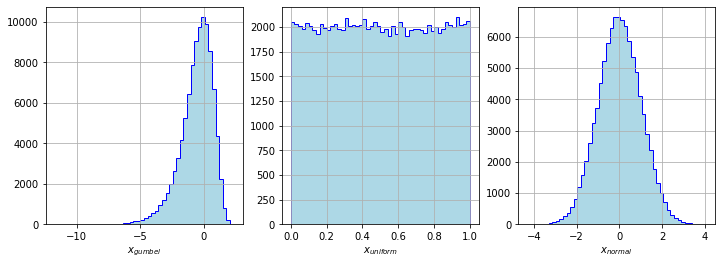
\includegraphics[width=0.9\linewidth]{figures/ex_gumbel_to_gauss.png}
\end{center}
\end{figure}
\end{solution}

\begin{question}
Without using the corresponding \texttt{rvs()} method try to generate 10 random numbers distributed as a Beta distribution with parameters \texttt{a=3} and \texttt{b=10}.

\noindent\textbf{Hint:} starts with generating uniformly distributed random numbers.
\end{question}	

\cprotEnv\begin{solution}
\begin{ipython}
from scipy.stats import beta, uniform

x = uniform.rvs(size=10)
b = beta(a=3, b=10)
x_b = b.ppf(x)

print (x_b)
\end{ipython}
\begin{ioutput}
[0.29190237 0.45669406 0.10336582 0.5403107 0.08305872 0.32425694
0.43902811 0.11820592 0.28659784 0.22316621]
\end{ioutput}
\end{solution}

\begin{question}
Consider two companies whose default probabilities as a function of time are modeled according to a log-normal distribution with $\sigma=0.5$ (\texttt{scipy.stats.lognorm(0.5)}). Compare the joint 2D distributions in case of no correlation and with a Gaussian correlation of 0.8.

\noindent\textbf{Hint:} to plot the joint distribution use \texttt{matplotlib} function \texttt{hist2d(x1, x2, range=[[x1min, x1max], [xmin, x2max]], bins=(50, 50)) }.
\end{question}

\cprotEnv\begin{solution}
\begin{ipython}
from scipy.stats import lognorm, multivariate_normal, norm
import numpy

numpy.random.seed(1)
samples = 1000000
l1_uncorr = lognorm(0.5).rvs(size=samples)
l2_uncorr = lognorm(0.5).rvs(size=samples)
mvnorm = multivariate_normal(mean = (0, 0), 
                             cov = [[1, 0.8],
                                    [0.8, 1]])
x = mvnorm.rvs(size=samples)
x_corr = norm.cdf(x)
l1_corr = lognorm(0.5).ppf(x_corr[:, 0])
l2_corr = lognorm(0.5).ppf(x_corr[:, 1])

plt.figure(figsize=(12, 4))
sub1 = plt.subplot(1, 2, 1)
sub1.hist2d(l1_uncorr, l2_uncorr, range=[[0, 2], [0, 2]], bins=(100, 100))
sub2 = plt.subplot(1, 2, 2)
sub2.hist2d(l1_corr, l2_corr, range=[[0, 2], [0, 2]], bins=(100, 100))
plt.show()
\end{ipython}
\noindent 
The resulting comparison is shown in Fig.~\ref{fig:joint_2d}.
\begin{figure}[htbp]
\begin{center}
	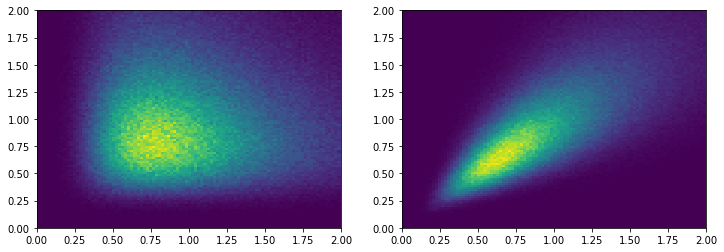
\includegraphics[width=0.9\linewidth]{figures/copula_lognormal.png}
\end{center}
\caption{Comparision of the joint 2D distributions in case of no correlation (left) and with a Gaussian correlation of 0.8 (right).}
\label{fig:joint_2d}
\end{figure}

In order to quantify the difference between the two cases, calculate the probability that both companies default in the next six months.

The probability that a single company defaulted in six months regardless the other can be calculated from the \texttt{cdf} of the log-normal distribution. Hence in case of independent probabilities is just required the squared of this value (about 0.07\%).

\begin{ipython}
default_6m = lognorm(0.5).cdf(.5)
print(default_6m**2)
\end{ipython}
\begin{ioutput}
0.006860563560014724
\end{ioutput}

In case of correlation instead we have to loop over the samples from the joint multivariate distribution and check how many times both values are less than \texttt{default\_6m}. Here two approaches are shown: the traditional one with a for-loop and a \emph{one-liner} using \texttt{numpy.array}.

\begin{ipython}
#success = 0.0
#for i in range(samples):
#    if max(x_corr[i]) < default_6m:
#        success += 1

success = len(x_corr[np.max(x_corr, axis=1) < default_6m])
print (success/samples)
\end{ipython}
\begin{ioutput}
0.044654
\end{ioutput}

This result can be interpreted graphically by saying that the entries in the "square" $[0, 0.5]$ in the left histogram are about 0.7\% of the total while the entries in the right plot in same "square" are about 4.5\% of the total. 
\end{solution}

\begin{question}
Imagine a risk manager which owns two non-investment graded bonds (e.g. rated BB+ and BB respectively). The bonds have been issued by two companies and their yearly default probabilities ($P_{\mathrm{def}}$) are as listed below:

\begin{table}[htbp]
\centering
\begin{tabular}{|c|c|c|}
\hline
Time & $P_{\mathrm{def}}$ Asset 1 & $P_{\mathrm{def}}$ Asset 2 \\
\hline
\hline
1 & 0.065 & 0.238 \\
2 & 0.081 & 0.152 \\
3 & 0.072 & 0.113 \\
4 & 0.064 & 0.092 \\
5 & 0.059 & 0.072 \\
\hline
\end{tabular}
\end{table}

How can a a copula be constructed to estimate the joint default probability of these two companies in the next year, assuming a Gaussian default correlation of $\rho_M = 0.4$ ?
\end{question}

\cprotEnv\begin{solution}
It is possible to map the cumulative default probabilities of each asset to the standard normal distribution via $F^{-1}[Q(t)]$.
\texttt{cumsum} can be used to determine $Q(t)$ from the inputs.

\begin{ipython}
import numpy as np
from scipy.stats import norm

PDF1 = np.array([0.065, 0.081, 0.072, 0.064, 0.059])
PDF2 = np.array([0.238, 0.152, 0.113, 0.092, 0.072])

C1 = PDF1.cumsum()
C2 = PDF2.cumsum()

for c in C1:
    print (f"{c:.3f} -> {norm.ppf(c):.4f}")
print ("")
for c in C2:
    print (f"{c:.3f} -> {norm.ppf(c):.4f}")
\end{ipython}
\begin{ioutput}
0.065 -> -1.5141
0.146 -> -1.0537
0.218 -> -0.7790
0.282 -> -0.5769
0.341 -> -0.4097

0.238 -> -0.7128
0.39 -> -0.2793
0.503 -> 0.0075
0.595 -> 0.2404
0.667 -> 0.4316
\end{ioutput}

\begin{table}[htbp]
\centering
\begin{tabular}{|c|c|c|c|c|c|c|}
\hline
Time & $P_{\mathrm{def}}$ Asset 1 & $Q_{\textrm{BB+}}(t)$ & $F^{-1}[Q_{\textrm{BB+}}(t)]$ & $P_{\mathrm{def}}$ Asset 2 & $Q_{\textrm{BB}}(t)$ & $F^{-1}[Q_{\textrm{BB}}(t)]$\\[5 pt]
\hline
\hline
1 & 0.065 & 0.065 & -1.5141 & 0.238 & 0.238 & -0.7128\\
2 & 0.081 & 0.146 & -1.0537 & 0.152 & 0.39 & -0.2793\\
3 & 0.072 & 0.218 & -0.7790 & 0.113 & 0.503 & 0.0075\\
4 & 0.064 & 0.282 & -0.5769 & 0.092 & 0.595 & 0.2404\\
5 & 0.059 & 0.341 & -0.4097 & 0.072 & 0.667 & 0.4316\\
\hline
\end{tabular}
\end{table}

At this point we can apply the correlation structure $\rho_M$ of the Gaussian multivariate distribution ($M$) to the transformed marginals $F^{-1}[Q_{\textrm{BB+}}(t)]$ and $F^{-1}[Q_{\textrm{BB}}(t)]$.

The joint probability of both companies defaulting within one year can be calculated as

\begin{equation*}
Q(t_{\textrm{BB+}}\leq 1 \cap t_{\textrm{BB}}\leq 1) = M(X_{\textrm{BB+}}\leq -1.5141 \cap X_{\textrm{BB}}\leq -0.7128, \rho=0.4)
\end{equation*}

\begin{ipython}
from scipy.stats import multivariate_normal

g = multivariate_normal(mean=[0,0],
                        cov=[[1, 0.4],
                             [0.4, 1]])

print (g.cdf([-1.5141, -0.7128]))
\end{ipython}
\begin{ioutput}
0.03435364791840133
\end{ioutput}
\noindent
which results to be around 3.4\%. Figure~\ref{fig:copula_no_marginals} shows the joint probability distribution, the number we were looking for is given by the fraction of events delimited by the red lines with respect to the total.

\begin{figure}[htbp]
\centering
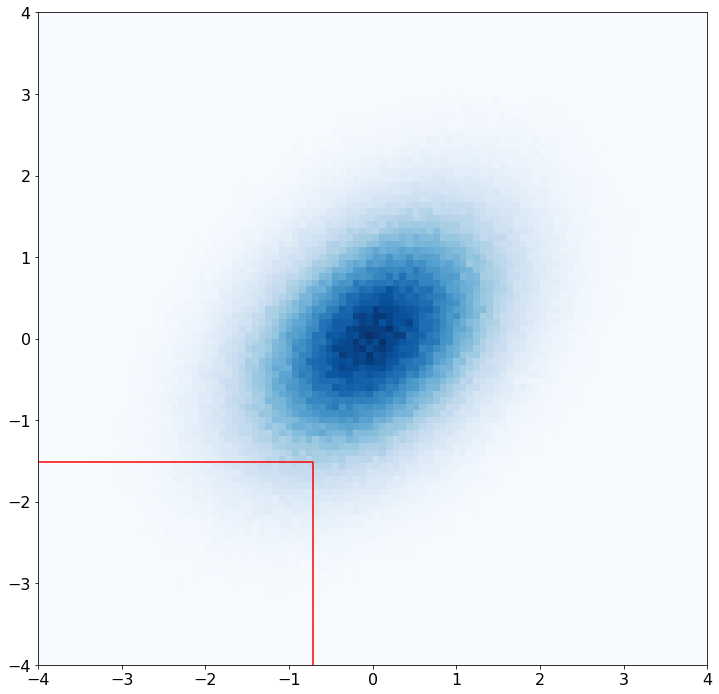
\includegraphics[width=0.5\linewidth]{figures/copula_no_marginals}
\caption{Multivariate Gaussian probability distribution with correlation $\rho=0.4$. The red lines delimited the area representing the default of the two companies within year one.}
\label{fig:copula_no_marginals}
\end{figure}
\end{solution}